\documentclass[17pt]{extarticle}
\usepackage{../mystyle}

\begin{document}

\section*{Работа №1}

Графики были построены с помощью \texttt{matplotlib} в Python.

\subsection*{a) \( F = -8x_1 + 3x_2 \to \min (\max) \)}

\[
    \begin{cases}
        x_1 + 2x_2 \leq 14   \\
        -4x_1 + 3x_2 \leq 12 \\
        x_1 \leq 6           \\
        x_1 \geq 0, \quad x_2 \geq 0
    \end{cases}
\]

\begin{figure}[H]
    \centering
    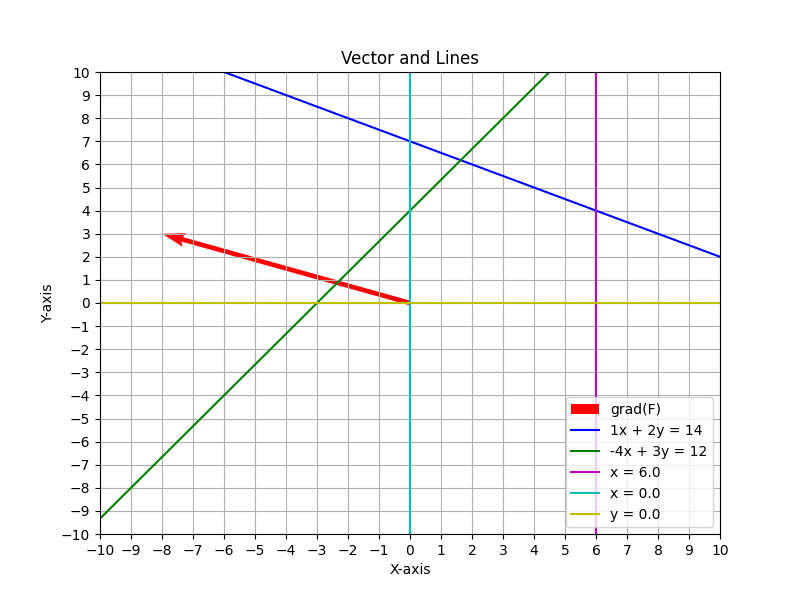
\includegraphics[width=0.7\textwidth]{a.png}
\end{figure}

\[
    F_{\min} = F(6, 0) = -48, \quad F_{\max} = F(0, 4) = 12
\]

\subsection*{b) \( F = 2x_1 + x_2 \to \min (\max) \)}

\[
    \begin{cases}
        2x_1 + x_2 \geq 10 \\
        -4x_1 + x_2 \leq 8 \\
        x_1 \geq 0, \quad x_2 \geq 0
    \end{cases}
\]

\begin{figure}[H]
    \centering
    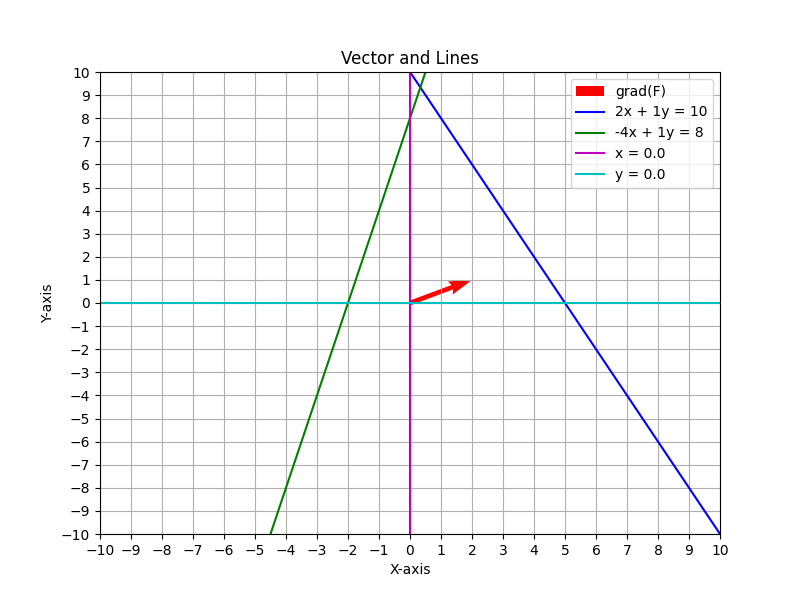
\includegraphics[width=0.7\textwidth]{b.png}
\end{figure}

\[
    F_{\min} = F(5, 0) = 10 \quad (\text{любая точка прямой } 2x + y = 10 \text{ подойдет, так как } \nabla F \text{ перпендикулярен ей})
\]
\[
    \nexists F_{\max}
\]

\subsection*{c) \( F = 2x_1 - x_2 \to \min (\max) \)}

\[
    \begin{cases}
        3x_1 - x_2 \geq 21 \\
        x_1 \leq 2         \\
        x_1 \geq 0, \quad x_2 \geq 0
    \end{cases}
\]

\begin{figure}[H]
    \centering
    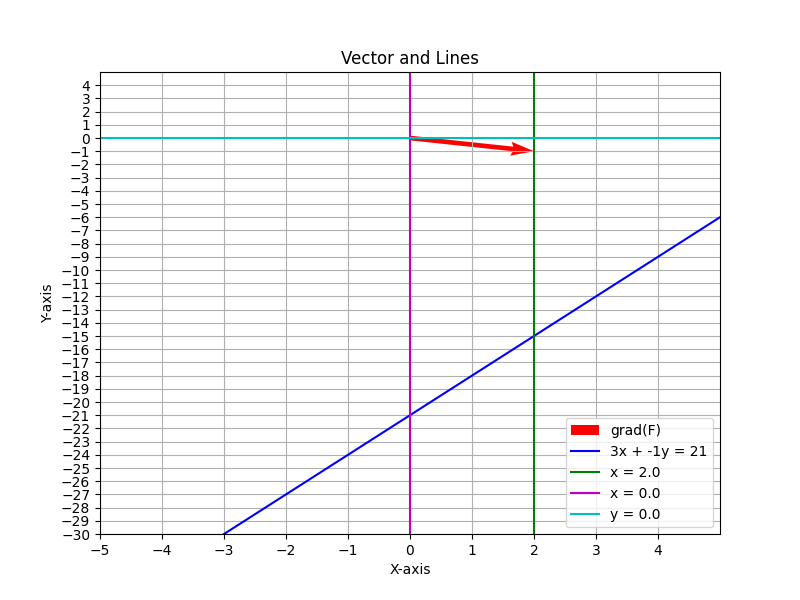
\includegraphics[width=0.7\textwidth]{c.png}
\end{figure}

\[
    \nexists F_{\min}, \quad \nexists F_{\max}, \quad \text{у системы вообще нет решений}
\]

\end{document}